\exercise

1. 研究下列函数在指定区间上的增减性:
\begin{tasks}(1)
    \task $f(x) = \tan \, x , \; (-\pi/2,\pi/2)$;
    \task $f(x) = \left(\arctan \, x\right) - x, \; \real$
\end{tasks}

(1) \solve 求导得
\begin{equation}
    \left(\tan \, x\right)^\prime = 1 + \left(\tan \, x\right)^2 > 0
\end{equation}
因此$\tan$在$(-\pi/2, \pi/2)$是增的.\qed\bigskip

(2) \solve 求导得
\begin{equation}
    \left(\left(\arctan \, x\right) - x\right)^\prime = \frac{1}{1+x^2} - 1 < 0
\end{equation}
因此函数$x \mapsto \left(\arctan \, x\right) - x$在$\real$是减的.\qed\bigskip

2. 证明不等式:
\begin{tasks}(2)
    \task $x(x-\arctan \, x) > 0 \; (x \neq 0)$;
    \task $x - \displaystyle\frac{x^2}{2}<\ln \, \left(1+x\right)<x \; (x>0)$;
    \task $x-\displaystyle\frac{x^3}{6}<\sin \, x < x \; (x > 0)$;
    \task $\ln \, \left(1+x\right)>\displaystyle\frac{\arctan \, x}{1+x} \left(x>0\right)$.
\end{tasks}

(1) \prove 由于该函数是奇的,故我们只讨论$x > 0$的情形,由于
\begin{equation}
    \left(0 - \arctan \, 0\right) = 0
\end{equation}
并且
\begin{equation}
    \left(x - \arctan \, x\right)^\prime = 1 - \frac{1}{1+x^2} > 0
\end{equation}
故对一切$x>0$都有
\begin{equation}
    \left(x - \arctan \, x\right) > 0
\end{equation}
又因为当$x > 0$时$x > 0$,故当$x > 0$时
\begin{equation}
    x \left(x - \arctan \, x\right) > 0
\end{equation}
有根据函数的奇偶性,得证当$x < 0$时也有
\begin{equation}
    x \left(x - \arctan \, x\right) > 0
\end{equation}
这就证明了对一切$x \neq 0$都有
\begin{equation}
    x \left(x - \arctan \, x\right) > 0.
\end{equation}
\qed\bigskip

(2) \prove 先证不等式右边,求导可知
\begin{equation}
    \left(\ln \, \left(1+x\right) - x\right)^\prime = \frac{1}{1+x} - 1 < 0 , \quad ( x > 0)
\end{equation}
并且
\begin{equation}
    \left(\ln \, \left(1+x\right) - x\right) \bigg\vert_{x = 0} = 0
\end{equation}
所以当$x > 0$时,恒有$\ln \, \left(1+x\right) - x < 0$,也就是$\ln \, \left(1+x\right) < x$.现在来证不等式左边,求导可知
\begin{equation}
    \left(x-\frac{x^2}{2}-\ln \, \left(1+x\right)\right)^\prime = 1 - x - \frac{1}{1+x}
\end{equation}
我们知道
\begin{align}
    &\mathrel{\phantom{\implies}} 1 - x^2 < 1 \\
    &\implies (1-x)(1+x) < 1 \\
    &\implies 1-x < \frac{1}{1+x} \, \quad (x > 0) 
\end{align}
所以有
\begin{equation}
    \left(x - \frac{x^2}{2}-\ln \, \left(1+x\right)\right)^\prime = 1 - x - \frac{1}{1+x} < 0
\end{equation}
又因为
\begin{equation}
    \left(x - \frac{x^2}{2}-\ln \, \left(1+x\right)\right) \bigg\vert_{x = 0} = 0
\end{equation}
所以对一切$x > 0$恒有
\begin{equation}
    x - \frac{x^2}{2} - \ln \, \left(1+x\right) < 0
\end{equation}
也就是
\begin{equation}
    x - \frac{x^2}{2} < \ln \, \left(1+x\right).
\end{equation}
\qed\bigskip

(3) \prove 我们只证不等式左边,由于在$x=0$处等号成立,故只需考虑导数的大小
\begin{align}
    &\mathrel{\phantom{\impliedby}} x - \frac{x^3}{6} < \sin \, x \\
    &\impliedby 1 - \frac{x^2}{2} < \cos \, x \\
    &\impliedby - x < -\sin \, x \\
    &\impliedby x > \sin \, x.
\end{align}
\qed\bigskip

(4) \prove 易知
\begin{align}
    &\mathrel{\phantom{\impliedby}} \ln \, \left(1+x\right) > \frac{\arctan \, x}{1+x} \\
    &\impliedby \ln \, \left(1+x\right) > \left(\arctan \, x\right) \left(\ln \, \left(1+x\right)\right)^\prime \\
    &\impliedby \frac{1}{\left(\ln \, \left(1+x\right)\right)^\prime} > \frac{\arctan \, x}{\ln \, \left(1+x\right)} \\
    &\impliedby \frac{\displaystyle\frac{1}{1+0}}{\displaystyle\frac{1}{1+x}} > \frac{\arctan \, x - \arctan \, 0}{\ln \, \left(1+x\right) - \ln \, \left(1+0\right)}
\end{align}
在区间$(0,x)$运用Cauchy定理可知
\begin{equation}
    \frac{\arctan \, x - \arctan \, 0}{\ln \, \left(1+x\right) - \ln \, \left(1+0\right)} = \frac{\displaystyle\frac{1}{1+\xi^2}}{\displaystyle\frac{1}{1+\xi}}, \quad \xi \in (0, x)
\end{equation}
毫无疑问$\displaystyle\frac{1}{1+\xi^2} < \displaystyle\frac{1}{1+0}$并且$\displaystyle\frac{1}{1+x}<\displaystyle\frac{1}{1+\xi}$,所以
\begin{equation}
    \displaystyle\frac{\displaystyle\frac{1}{1+\xi^2}}{\displaystyle\frac{1}{1+\xi}} < \displaystyle\frac{\displaystyle\frac{1}{1+0}}{\displaystyle\frac{1}{1+x}}
\end{equation}
所以
\begin{equation}
    \displaystyle\frac{\arctan \, x - \arctan \, 0}{\ln \, \left(1+x\right) - \ln \, \left(1+0\right)} < \displaystyle\frac{\displaystyle\frac{1}{1+0}}{\displaystyle\frac{1}{1+x}}
\end{equation}
所以
\begin{equation}
    \ln \, \left(1+x\right)>\frac{\arctan \, x}{1+x}.
\end{equation}
\qed\bigskip

3. 证明不等式
\begin{tasks}(1)
    \task 当$0<x_1<x_2<\pi/2$时,
    \begin{equation*}
        \frac{\tan x_2}{\tan x_1} > \frac{x_2}{x_1};
    \end{equation*}
    \task 当$x,y>0$且$\beta>\alpha>0$时,
    \begin{equation*}
        \left(x^\alpha + y^\alpha \right)^{1/\alpha} > \left(x^\beta + y^\beta\right)^{1/\beta};
    \end{equation*}
    \task 若$x>-1$,则
    \begin{align*}
        \left(1+x\right)^\alpha &\leq 1 + \alpha x \quad \left(0 < \alpha \leq 1\right), \\
        \left(1+x\right)^\alpha &\geq 1 + \alpha x \quad \left(\alpha < 0, \text{或} \; \alpha \geq 1\right)
    \end{align*}
    \task 设$p \geq 2$,当$x \in [0,1]$时,
    \begin{equation*}
        \left(\frac{1+x}{2}\right)^p + \left(\frac{1-x}{2}\right)^p \leq \frac{1}{2} \left(1+x^p\right).
    \end{equation*}
\end{tasks}

(1) \prove 易知
\begin{align}
    &\mathrel{\phantom{\impliedby}} \frac{\tan \, x_2}{\tan \, x_1} > \frac{x_2}{x_1} \\
    &\impliedby \frac{\tan \, x_1 + \tan \, x_2 - \tan \, x_1}{\tan \, x_1} > \frac{x_1 + x_2 - x_1}{x_1} \\
    &\impliedby 1 + \frac{\tan \, x_2 - \tan \, x_1}{\tan \, x_1} > 1 + \frac{x_2 - x_1}{x_1} \\
    &\impliedby \frac{\tan \, x_2 - \tan \, x_1}{\tan \, x_1} > \frac{x_2-x_1}{x_1} \\
    &\impliedby \frac{\tan \, x_2 - \tan \, x_1}{x_2 - x_1} > \frac{\tan \, x_1}{x_1}
\end{align}
现在让我们在区间$(x_1,x_2)$应用Lagrange定理,可知存在$\xi \in (x_1,x_2)$,使得
\begin{equation}
    \frac{\tan \, x_2 - \tan \, x_1}{x_2 - x_1} = 1 + \left(\tan \, \xi\right)^2 = \frac{1}{\left(\cos \, \xi\right)^2}
\end{equation}
注意到
\begin{equation}
    \frac{\tan \, x_1}{x_1} = \frac{\sin \, x_1}{x_1 \cos \, x_1} = \frac{1}{\displaystyle\frac{x_1}{\sin \, x_1} \cos \, x_1}
\end{equation}
由于
\begin{equation}
    \frac{x_1}{\sin \, x_1} > 1 \geq \cos \, \xi, \quad \cos \, x_1 > \cos \, \xi
\end{equation}
所以
\begin{equation}
    \frac{1}{\displaystyle\frac{x_1}{\sin \, x_1}\cos \, x_1} < \frac{1}{\left(\cos \, \xi\right)^2} 
\end{equation}
所以
\begin{equation}
    \frac{\tan \, x_2 - \tan \, x_1}{x_2 - x_1} > \frac{\tan \, x_1}{x_1}
\end{equation}
所以
\begin{equation}
    \frac{\tan \, x_2}{\tan \, x_1} > \frac{x_2}{x_1}.
\end{equation}
\qed\bigskip

(1) \prove (证法2:利用凸性)令
\begin{equation}
    f(x) = \tan \, x
\end{equation}
则
\begin{equation}
    f^\prime (x) = \frac{1}{\left(\cos x\right)^2}, \quad f^{\prime\prime}(x) = \frac{2\sin \, x}{\left(\cos \, x\right)^3} > 0, \quad (0 < x < \pi/2)
\end{equation}
由此可知$f$在$(0,\pi/2)$是严格凸的,所以对任意$0 < x_1 < x_2 < \pi/2$有
\begin{equation}
    \frac{f(x_1)-f(0)}{x_1-0} < \frac{f(x_2)-f(0)}{x_2-0}
\end{equation}
也就是
\begin{equation}
    \frac{\tan \, x_1}{x_1} < \frac{\tan \, x_2}{x_2}
\end{equation}
从而得
\begin{equation}
    \frac{\tan \, x_2}{\tan \, x_1} > \frac{x_2}{x_1}.
\end{equation}
\qed\bigskip

\annotate 凸性使证明一下子变得简洁了好多.\bigskip

(2) \prove 假设$x,y>1$,那么有
\begin{align}
    &\mathrel{\phantom{\impliedby}} \left(x^\alpha + y^\alpha\right) > \left(x^\beta + y^\beta \right)^\beta \\
    &\impliedby \text{函数} \; t \mapsto \exp \, \{ \frac{\ln \, \left(x^t + y^t \right)}{t}\} \; \text{是递减的}, \; (0 < t) \\
    &\impliedby \text{它的导数} \; \exp \, \{ \frac{\ln \, \left(x^t+y^t\right)}{t} \}\left(\frac{x^t\ln \, x + y^t \ln \, y}{t\left(x^t+y^t\right)} - \frac{\ln \, \left(x^t + y^t\right)}{t^2}\right) < 0 \\
    &\impliedby \frac{x^t\ln \, x + y^t \ln \, y}{t\left(x^t+y^t\right)} - \frac{\ln \, \left(x^t + y^t\right)}{t^2} < 0 \\
    &\impliedby \frac{x^t}{x^t+y^t} \ln \, \left(x^t\right) + \frac{y^t}{x^t+y^t} \ln \, \left(y^t\right) < \ln \, \left(x^t+y^t\right) \\
    &\impliedby \text{令} \; a = x^t, b = y^t, \lambda_1 = \frac{a}{a+b}, \lambda_2 = \frac{b}{a+b} \; \text{则} \; \lambda_1 \ln \, a + \lambda_2 \ln \, b < \ln \, \left(a+b\right) \\
    &\impliedby \exp \, \{\lambda_1 \ln \, a + \lambda_2 \ln \, b\} < \exp \, \{\ln \, \left(a+b\right)\} \\
    &\impliedby \text{利用凸性得} \; \exp \, \{\lambda_1 \ln \, a + \lambda_2 \ln \, b\} < \lambda_1  \exp \, \{ \ln \, a \} + \lambda_2 \exp \, \{ \ln \, b \} \\
    &\mathrel{\phantom{\impliedby}} = \lambda_1 a + \lambda_2 b < a+b = \exp \, \{\ln \, \left(a+b\right)\}.
\end{align}
\qed\bigskip

\annotate 这充分体现了导数工具的强大.\bigskip

(3) \prove 当$(0<\alpha\leq 1)$时
\begin{align}
    &\mathrel{\phantom{\impliedby}} \left(1+x\right)^\alpha \leq 1 + \alpha x \\
    &\impliedby \exp \, \{ \alpha \ln \, \left(1+x\right) \} \leq \exp \, \{ \ln \, \left( 1+\alpha x \right) \} \\
    &\impliedby \alpha \ln \, \left(1+x\right) \leq \ln \, \left(1+\alpha x\right) \\
    &\impliedby \frac{\ln \, \left(1+1\cdot x\right)}{1} \leq \frac{\ln \, \left(1+\alpha x\right)}{\alpha}
\end{align}
好戏来了!令
\begin{equation}
    g(t) = \frac{\expe^t - 1}{x} , \quad (x \; \text{是常数})
\end{equation}
再令
\begin{equation}
    t_1 = \ln \, \left(1+\alpha x\right), \quad t_2 = \ln \, \left(1+ 1 \cdot x\right)
\end{equation}
那么利用函数$g$的凸性立刻有
\begin{equation}
    \frac{g(t_2)-g(0)}{t_2-0} \geq \frac{g(t_1) - g(0)}{t_1 - 0}
\end{equation}
整理得
\begin{equation}
    \frac{1}{\ln \, \left(1+x\right)} \geq \frac{\alpha}{\ln \, \left(1+\alpha x\right)}
\end{equation}
注意到这里的$\ln \, \left(1+x\right), \ln \, \left(1+\alpha x\right)$都是负的所以乘的时候要变号,所以
\begin{align}
    &\mathrel{\phantom{\implies}} \frac{1}{\ln \, \left(1+x\right)} \geq \frac{\alpha}{\ln \, \left(1+\alpha x\right)} \\
    &\implies 1 \leq \frac{\alpha \ln \, \left(1+x\right)}{\ln \, \left(1+\alpha x\right)} \\
    &\implies \ln \, \left(1+\alpha x\right) \geq \alpha \ln \, \left(1+x\right) \\
    &\implies \left(1+x\right)^\alpha \leq 1 + \alpha x.
\end{align}
等号当$\alpha = 1$时成立.\qed\bigskip

\annotate 至于我是怎么样想到要构造那个函数$g(t) = \displaystyle\frac{\expe^t-1}{x}$的呢?其实在出现$\displaystyle\frac{\ln \, \left(1+1 \cdot x\right)}{1} \leq \displaystyle\frac{\ln \, \left(1+\alpha\right)}{\alpha}$的时候可能会令人联想到要把$\{ (t, \displaystyle\frac{\ln \, \left(1+xt\right)}{t}) : 0 \leq t \leq 1\}$画出来,然后那个$g$就是这个函数的反函数,所以利用$g$的凸性就顺理成章了.\bigskip

(4) \prove 令
\begin{align}
    f(x) &= \left(\frac{1+x}{2}\right)^p + \left(\frac{1-x}{2}\right)^p \\
    g(x) &= \frac{1}{2} \left(1+x^p\right)
\end{align}
求导得
\begin{align}
    f^\prime (x) &= \frac{1}{2}p\left(\left(\frac{1+x}{2}\right)^{p-1}-\left(\frac{1-x}{2}\right)^{p-1}\right) > 0 \\
    g^\prime (x) &= \frac{1}{2}px^{p-1} > 0
\end{align}
我们发现由于$p \geq 2$所以
\begin{equation}
    f(0) = 2 \left(\frac{1}{2}\right)^p \leq g(0) = \frac{1}{2}
\end{equation}
现在要使得$f(x) \leq g(x)$对一切$x \in [0,1]$成立,只要再确保$f$在此区间内增长得比$g$「更加慢」就可以了,也就是要保证
\begin{align}
    &\mathrel{\phantom{\impliedby}} f^\prime (x) \leq g^{\prime} (x) \\
    &\impliedby \left(\frac{1+x}{2}\right)^{p-1} - \left(\frac{1-x}{2}\right)^{p-1} \leq x^{p-1} = \left(\frac{2x}{2}\right)^{p-1} \\
    &\impliedby \left(\frac{1+x}{2}\right)^{p-1} = \left(\frac{1-x}{2} + \frac{2x}{2}\right)^{p-1} \leq \left(\frac{1-x}{2}\right)^{p-1} + \left(\frac{2x}{2}\right)^{p-1} \label{eq:3-5-76}
\end{align}
而不等式\ref{eq:3-5-76}由函数$x \mapsto \left(x\right)^{p-1}$的凸性得到保证,而函数$x \mapsto \left(x\right)^{p-1}$的凸性相应地由$p \geq 2$得到保证.\qed\bigskip

4. 设函数$f$在$[0,1]$上有三阶导函数,且$f(0)=f(1)=0$.令$F(x)=x^2 f(x)$,求证:存在$\xi \in (0,1)$,使得$F^{\prime\prime\prime}(\xi)=0$.

\prove 由于
\begin{equation}
    F(0) = 0^2 f(0) = 0, \quad F(1) = 1^2 f(1) = f(1) = 0
\end{equation}
所以可在区间$(0,1)$对$F$应用Rolle定理,可知存在$\xi_1 \in (0,1)$使得
\begin{equation}
    F^{\prime}(\xi_1) = 0
\end{equation}
我们还知道
\begin{equation}
    F^\prime (x) = 2x f(x) + x^2 f^{\prime} (x) \implies F^\prime (0) = 0
\end{equation}
所以可在区间$(0, \xi_1)$对$F^\prime$应用Rolle定理,可知存在$\xi_2 \in (0, \xi_1)$使得
\begin{equation}
    F^{\prime\prime}(\xi_2) = 0
\end{equation}
我们还知道
\begin{equation}
    F^{\prime\prime}(x) = 2f(x) + 2xf^{\prime}(x) + 2x f^{\prime}(x) + x^2 f^{\prime\prime}(x) \implies F^{\prime\prime}(0) = 0
\end{equation}
所以可在区间$(0, \xi_2)$对$F^{\prime\prime}$应用Rolle定理,可知存在$\xi_3 \in (0, \xi_2)$使得
\begin{equation}
    F^{\prime\prime\prime}(\xi_3) = 0.
\end{equation}
\qed\bigskip

5. 设函数$f$在区间$[0,+\infty)$上可导,$f(0)=0$,且$f^\prime$严格递增.求证:$f(x)/x$在$(0,+\infty)$上也严格递增.

\prove 任取$x_1, x_2 \in (0, +\infty), x_1 < x_2$,那么由$f$的凸性我们有
\begin{equation}
    \frac{f(x_1)-f(0)}{x_1 - 0} < \frac{f(x_2)-f(0)}{x_2-0}
\end{equation}
也就是
\begin{equation}
    \frac{f(x_1)}{x_1} < \frac{f(x_2)}{x_2}
\end{equation}
这就说明$f(x)/x$在$[0,+\infty)$是递增的.\qed\bigskip

6. 设函数$f$在$\real$上有界且$f^{\prime\prime} \geq 0$.证明:$f$为常值函数.

\prove 不妨设$f$在$x_0$处取得最大值$M$也就是说$f(x_0) = M$,那么对任意$x_1 \in (-\infty, x_0)$,有
\begin{align}
    &\mathrel{\phantom{\implies}} f(x_0) \geq f(x_1) \\
    &\implies f(x_0)-f(x_1) \geq 0 \\
    &\implies \frac{f(x_0)-f(x_1)}{x_0-x_1} \geq 0 
\end{align}
在区间$(x_1,x_0)$应用Lagrange定理可知存在$x_2 \in (x_1,x_0)$使得
\begin{equation}
f^{\prime}(x_2) = \displaystyle\frac{f(x_0)-f(x_1)}{x_0-x_1} \geq 0
\end{equation}
而依Fermat定理,在$x_0$处有$f^{\prime}(x_0) = 0$.因此只能是$f^{\prime}(x_2) = 0$,否则若$f^{\prime}(x_2) > 0$,在区间$(x_2,x_0)$对$f^\prime$应用Lagrange定理可知存在$x_3 \in (x_2,x_0)$满足
\begin{equation}
    f^{\prime\prime}(x_3) = \frac{f^{\prime}(x_0)-f^{\prime}(x_2)}{x_0-x_2} < 0
\end{equation}
这与$f^{\prime\prime} \geq 0$矛盾.同理可证,对任意$x > x_0$都有$f^{\prime}(x) = 0$.由于$f^\prime = 0$所以$f$是常的.\qed\bigskip

7. 设函数$f$和$g$在区间$[a,+\infty)$上连续,且当$x>a$时$\left| f^{\prime}(x) \right| \leq g^{\prime}(x)$.证明:当$x \geq a$时,
\begin{equation*}
    \left| f(x) - f(a) \right| \leq g(x) - g(a).
\end{equation*}

\prove 当$x=a$时关系式显然成立,当$x>a$时,令$d = x-a$,对任意$n \in \nat$,有
\begin{align}
    &\mathrel{\phantom{\impliedby}} \left| f(x) - f(a) \right| \leq g(x) - g(a) \\
    &\impliedby \left| \sum_{i=1}^n \left(f(a+\frac{i}{n} d) - f(a + \frac{i-1}{n}d) \right) \right| \leq \sum_{i=1}^n \left( g(a+\frac{i}{n}d) - g(a+\frac{i-1}{n}d) \right) \\
    &\impliedby \sum_{i=1}^n \left| f(a + \frac{i}{n} d) - f(a+ \frac{i-1}{n} d)\right| \leq \sum_{i=1}^n \left(g(a + \frac{i}{n} d) - g(a + \frac{i-1}{n} d)\right) \\
    &\impliedby \sum_{i=1}^n \left| \frac{d}{n} \cdot \frac{f(a+ \displaystyle\frac{i}{n} d) - f(a+ \displaystyle\frac{i-1}{n} d)}{\displaystyle\frac{d}{n}}\right| \leq \sum_{i=1}^n \left(\frac{d}{n} \cdot \frac{g(a + \displaystyle\frac{i}{n} d) - g(a + \displaystyle\frac{i-1}{n} d)}{\displaystyle\frac{d}{n}}\right)
\end{align}
由于$\left| f^{\prime} (x)\right| \leq g^{\prime} (x)$,故存在足够大的$N \in \nat$,使得当$n \geq N$时,对任意$1 \leq i \leq n$,都有
\begin{equation}
    \left| \frac{f(a + \displaystyle\frac{i}{n} d) - f(a + \displaystyle\frac{i-1}{n} d)}{\displaystyle\frac{d}{n}} \right| \leq \frac{g(a + \displaystyle\frac{i}{n} d) - g(a + \displaystyle\frac{i-1}{n} d)}{\displaystyle\frac{d}{n}}.
\end{equation}
\qed\bigskip

8. 证明:当$x>0$且$x\neq 1$时,有
\begin{equation*}
    \left(1-x\right)\left(x^2 \expe^{1/x}-\expe^{x}\right) > 0.
\end{equation*}

\prove 设$\beta_1, \beta_2 > 0$且满足$\beta_1 + \beta_2 = \displaystyle\frac{1}{x^2}$.那么当$0 < x < 1$时
\begin{align}
    &\mathrel{\phantom{\impliedby}} \left(1-x\right)\left(x^2 \expe^{1/x} - \expe^x\right) > 0  \\
    &\impliedby x^2 \expe^{1/x} - \expe^{x} > 0 \\
    &\impliedby x^2 \expe^{1/x} > \expe^{x} \\
    &\impliedby \frac{\exp \, \{ 1/x \}}{1/x^2} > \exp \, \{ \frac{1/x}{1/x^2} \} \\
    &\impliedby \frac{\exp \, \{ \beta_1 x + \beta_2 x\}}{\beta_1 + \beta_2} > \expe \, \{ \frac{\beta_1 x + \beta_2 x}{\beta_1 + \beta_2} \} \label{eq:3-5-98}
\end{align}
不等式\ref{eq:3-5-98}由函数$\exp$的凸性得到保证.当$x > 1$时,令$t = \displaystyle\frac{1}{x}$,则有
\begin{align}
    &\mathrel{\phantom{\impliedby}} \left(1-x\right)\left(x^2 \expe^{1/x} - \expe^x\right) > 0  \\
    &\impliedby x^2 \expe^{1/x} - \expe^{x} < 0 \\
    &\impliedby \frac{1}{t^2} \expe^t - \expe^{1/t} < 0 \\
    &\impliedby \expe^t - t^2 \expe^ - t^2 \expe^{1/t} < 0 \\
    &\impliedby t^2 \expe^{1/t} - \expe^t > 0. \label{eq:3-5-103}
\end{align}
而不等式\ref{eq:3-5-103}正好是已经证明过的情形.\qed\bigskip

9. 求下列函数的最大值和最小值:
\begin{tasks}(2)
    \task $f(x) = x^4 - 2x^2 + 5 \; (\left| x \right| \leq 2)$; 
    \task $f(x) = \left(\sin \, 2x\right) - x \; \left( \left| x \right| \leq \pi / 2\right)$;
    \task $f(x) = x \ln \, x \; \left(x > 0\right)$;
    \task $f(x) = x^2 - 3x + 2 \; \left(x \in \real\right)$;
    \task $f(x) = \left| x^2 - 3x + 2 \right| \left(\left| x \right| \leq 10\right)$;
    \task $f(x) = \arctan \, \displaystyle\frac{1-x}{1+x} \; \left(0 \leq x \leq 1\right)$.
\end{tasks}

(1) \solve 令$x(t)=\sqrt{t}$,问题等价于求
\begin{equation}
    f(x(t)) = t^2 - 2t + 5, \quad \left(0 \leq t \leq 4\right)
\end{equation}
的最值.先考虑边界点$t = 0$与$t=4$:
\begin{equation}
    f(x(0)) = 5, \quad f(x(4)) = 13
\end{equation}
求$f \circ x$关于$t$的导数得
\begin{equation}
    \left(f \circ x\right)^{\prime} (t) = 2t - 2 \implies \left(f \circ x\right)^{\prime} (1) = 0
\end{equation}
再求$f \circ x$关于$t$的二阶导数得
\begin{equation}
    \left(f \circ x\right)^{\prime\prime} = 2 > 0
\end{equation}
可知$t = 1$是$f \circ x$的极小值点.故极小值为
\begin{equation}
    f(x(1)) = 1 - 2 + 5 = 4
\end{equation}
比较可知极大值为$f(x(4))=13$.\qed\bigskip

(2) \solve 令$t = 2x$,问题等价于求
\begin{equation}
    g(t) = \left(\sin \, t\right) - \frac{t}{2}, \quad \left(-\pi \leq t \leq \pi\right)
\end{equation}
的最值.为判断$g$的增减性们求导:
\begin{equation}
    g^{\prime}(t) = \left(\cos \, t\right) - \frac{1}{2} 
\end{equation}
由此可知
\begin{equation}
g^{\prime}(-\pi) = -3/2, \quad g^{\prime}(-\pi/2) = -1/2, \quad g^{\prime}(0) = 1/2, \quad g^{\prime\prime}(\pi/2) = -1/2, \quad g^{\prime}(\pi) = -3/2
\end{equation}
由此可知,存在$x_0 \in (-\pi / 2, 0), x_1 \in (0, \pi / 2)$使得$g^{\prime}(x_0) = 0, g^{\prime}(x_1) = 0$,并且由$\cos$的严格单调性可知这样的$x_0, x_1$是唯一的.由三角函数的性质
\begin{equation}
-1 < \sin \, x_0 < 0, \quad 0 < \sin \, x_1 < 1
\end{equation}
故
\begin{equation}
-1/2 < g(x_0) < 1/2, \quad 1/2 < g(x_1) < 3/2
\end{equation}
而
\begin{equation}
    g(-\pi) = -\pi / 2, \quad g(\pi) = \pi / 2
\end{equation}
显然$\pi/2 > 3/2$故$g(\pi) = \pi/2$为最大值,而又由于$-\pi/2 < -1/2$,故$g(-\pi) = -\pi/2$为最小值.\qed\bigskip

(3) \solve 求导得
\begin{align}
    f^{\prime}(x) &= \left(\ln \, x\right) + 1 \\
    f^{\prime\prime}(x) &= \frac{1}{x} > 0, \quad (x > 0)
\end{align}
由对数函数的性质可知$\ln \, \left(\expe^{-1}\right) = - \ln \, \expe = -1$可知$f^{\prime}(\expe^{-1}) = -1 + 1 = 0$,可知$x = \expe^{-1}$是$f^{\prime}(x) = 0$的一个解.又因为$f^{\prime\prime}$严格大于$0$,可知$f^{\prime}$有严格单调性,从而$x=\expe^{-1}$是$f^{\prime}$的唯一实根.又因为$f^{\prime\prime}(\expe^{-1}) > 0$可知$x = \expe^{-1}$是$f$的一个极小值点.

又因为
\begin{equation}
    \lim_{x \to 0^+} x \ln \, x = 0, \quad \lim_{x \to +\infty} x \ln \, x = +\infty
\end{equation}
并且$f(\expe^{-1}) = \expe^{-1} \ln \, \left(\expe^{-1}\right) = -\expe^{-1} < 0$,可知$f$的最下值是$f(\expe^{-1}) = -\expe^{-1}$,而最大值为$+\infty$(或不存在).\qed\bigskip

(4) \solve 配方得
\begin{align}
    f(x) &= (x - \frac{3}{2})^2 - \frac{1}{4}
\end{align}
因此最大值为$+\infty$,最小值为$-\displaystyle\frac{1}{4}$.\qed\bigskip

(5) \solve 配方得
\begin{align}
    f(x) &= \left| \left(x - \frac{3}{2}\right)^2 - \frac{1}{4} \right|
\end{align}
因此最小值为$0$.现在比较两个端点处的函数值:
\begin{equation}
    f(-10) = 132, \quad f(10) = 72
\end{equation}
因此最大值为$132$.\qed\bigskip

(6) \solve 求导得
\begin{align}
    f^{\prime}(x) &= \left(\arctan \, \displaystyle\frac{1-x}{1+x}\right)^{\prime} \\
    &= \displaystyle\frac{1}{1+\left(\displaystyle\frac{1-x}{1+x}\right)^2} \left(\displaystyle\frac{1-x}{1+x}\right)^{\prime} \\
    &= \displaystyle\frac{1}{1+\left(\displaystyle\frac{1-x}{1+x}\right)^2} \left(\left(-1\right)\left(\frac{1}{1+x}\right)+\left(1-x\right)\left(\displaystyle\frac{1}{1+x}\right)^{\prime}\right) \\
    &= \displaystyle\frac{1}{1+\left(\displaystyle\frac{1-x}{1+x}\right)^2} \left(-\displaystyle\frac{1}{1+x}+\left(1-x\right)\left(-\displaystyle\frac{1}{\left(1+x\right)^2}\right)\right) \\
    &= -\frac{\left(1+x\right)^2}{\left(1-x\right)^2+\left(1+x\right)^2} \left(\frac{1}{1+x} + \frac{1-x}{\left(1+x\right)^2}\right) = - \frac{1+x+1-x}{\left(1-x\right)^2+\left(1+x\right)^2} \\
    &= -\frac{1}{1+x^2}
\end{align}
由此可知
\begin{equation}
    \left(f(x) + \arctan \, x\right)^{\prime} = 0
\end{equation}
由此可知存在常数$C \in \real$,使得对一切$x \in [0,1]$都有
\begin{equation}
    f(x) + \arctan \, x = C
\end{equation}
取$x = 0$,则
\begin{equation}
    C = f(0) + \arctan \, 0 = f(0) = \arctan \, 1 = \frac{\pi}{4}
\end{equation}
这样就把$C$解了出来,现在我们知道了
\begin{equation}
    f(x) = C - \arctan \, x = \frac{\pi}{4} - \arctan \, x
\end{equation}
这样我们就知道了最小值为$f(1) = \displaystyle\frac{\pi}{4} - \arctan \, 1 = 0$,最大值为$f(0) = \displaystyle\frac{\pi}{4} - \arctan \, 0 = \displaystyle\frac{\pi}{4}$.\qed\bigskip

10. 质量为$W$的物体放在一粗糙的平面上,对它施加一个力以克服摩擦,使它在平面上滑动.设摩擦系数为$\mu$,问该力与水平面成何角度,方可使力最小?

\solve 设施加的力的大小是$F$,与平面的夹角为$\theta$,设摩擦力为$F_{R}$,设重力为$F_{G}$,设$g$是重力加速度,于是我们有
\begin{equation}
    \begin{cases}
        F_{G} = Wg \\
        F_{R} = \mu \left(Wg - F \sin \, \theta\right) 
    \end{cases}
\end{equation}
要让拉力刚好抵消摩擦力,应有
\begin{equation}
    F_{R} = F \cos \, \theta \implies F \cos \, \theta = \mu Wg - \mu F \sin \, \theta \implies F = \frac{\mu W g}{\cos \theta + \mu \sin \, \theta}
\end{equation}
最小化$F$等价于最大化$\cos \, \theta + \mu \sin \, \theta$,令$g(\theta) = \cos \, \theta + \mu \sin \, \theta$,对$g$求导得
\begin{equation}
    g^{\prime}(\theta) = - \sin \, \theta + \mu \cos \, \theta
\end{equation}
对$g^{\prime}$置零得
\begin{equation}
    - \sin \, \theta + \mu \cos \, \theta = 0 \implies \mu = \frac{\sin \, \theta}{\cos \, \theta} = \tan \, \theta
\end{equation}
由此得$\theta = \arctan \, \mu$,又因为
\begin{equation}
    g^{\prime\prime}(\theta) = - \cos \, \theta - \mu \sin \, \theta < 0
\end{equation}
所以$\theta = \arctan \, \mu$是极大值点.所以当$\theta = \arctan \, \mu$时力$F$最小.\qed\bigskip

\begin{figure}[H]
    \centering
    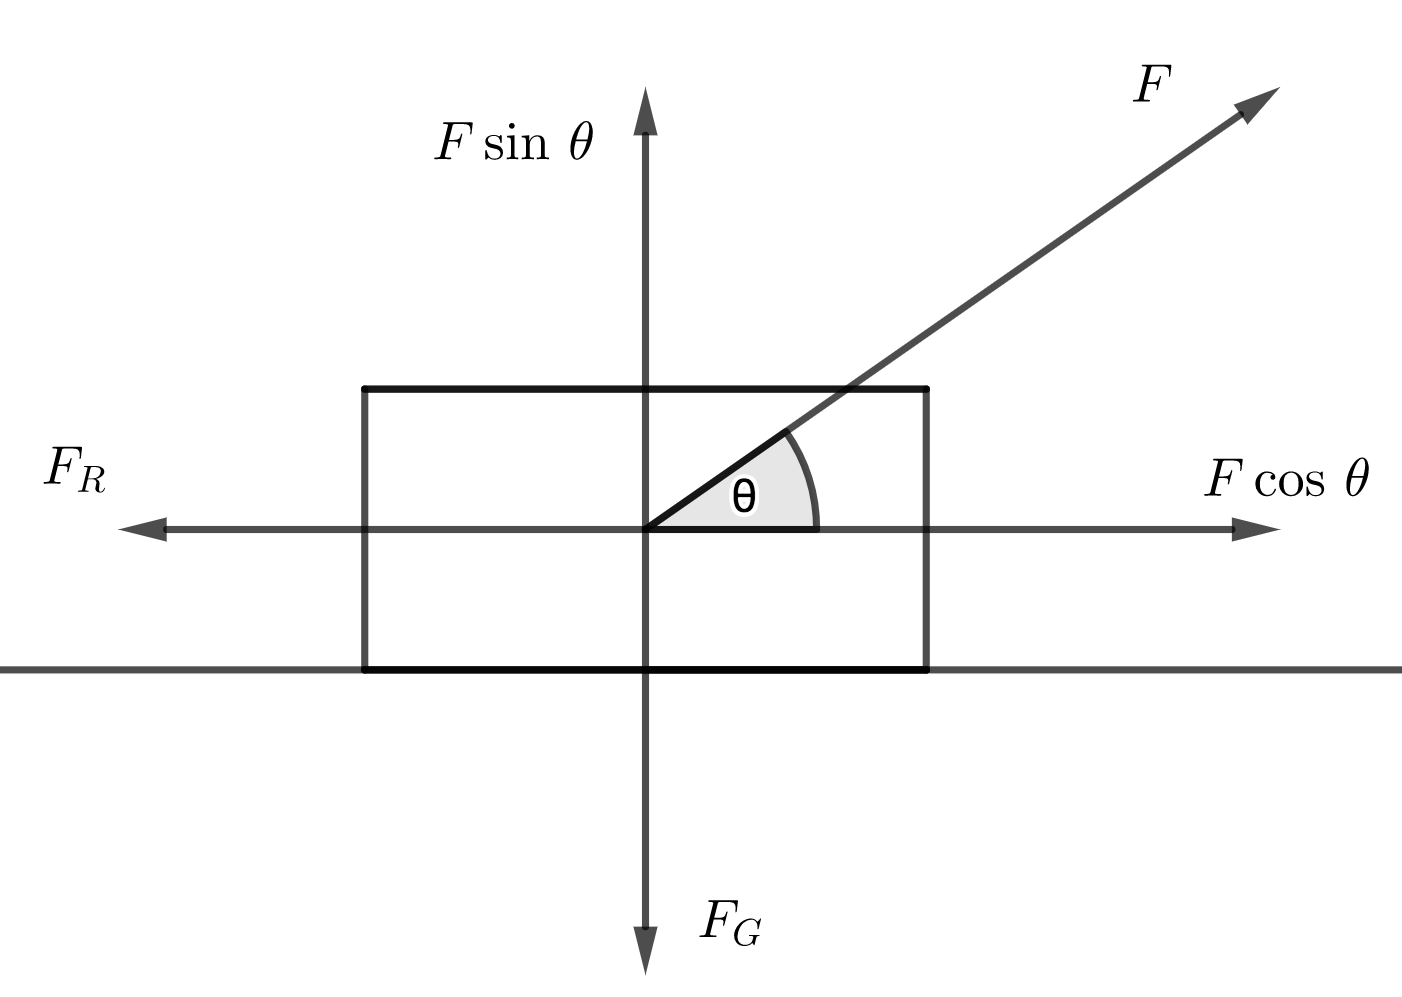
\includegraphics[width=0.45\textwidth]{chapter3/force.png}
    \caption{题10受力分析图}
\end{figure}